\documentclass[a4paper,12pt,titlepage]{report}
\usepackage[utf8]{inputenc}
\usepackage{graphicx}

\usepackage[footnotesize]{caption}

\makeatletter
\renewcommand{\fnum@figure}{\small\textbf{\figurename~\thefigure}}
\makeatother

\setcounter{secnumdepth}{-1} 

% Title Page
\title{Assignment Network Simulation}
\author{Peter De Wolf \& Wout Vekemans}
\begin{document}
\begin{titlepage}
	\maketitle
	\thispagestyle{empty}
\end{titlepage}

\section{Exercise 1: Bandwidth restrictions on Kotnet}
\begin{enumerate}
 \item When we leave out the uploading connection, the throughput of the download connection is relatively constant. See figure \ref{noUpload}. Sometimes a packet gets lost, decreasing the throughput. This is caused by full buffers, because the the connection between the server and the router is slower than the server interconnection (4 Mbps vs 100 Mbps).
  \begin{figure}[!h]
\centering
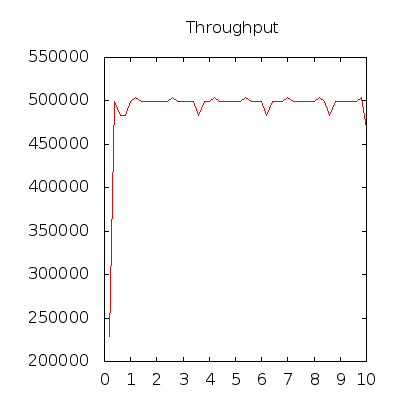
\includegraphics[width=0.5\textwidth]{noUpload.png}
\caption{Throughput of the main FTP connection}
\label{noUpload}
\end{figure}
\item When re-enabling the uploading connection, we see 
\end{enumerate}


\end{document}          
